%============================================================================
% tento soubor pouzijte jako zaklad
% (c) 2008 Michal Bidlo
% E-mail: bidlom AT fit vutbr cz
%============================================================================
% kodovaní: iso-8859-2 (zmena prikazem iconv, recode nebo cstocs)
%----------------------------------------------------------------------------
% zpracování: make, make pdf, make desky, make clean
% připomínky posílejte na e-mail: bidlom AT fit.vutbr.cz
% vim: set syntax=tex encoding=latin2:
%============================================================================
\documentclass[english,print]{fitthesis} % odevzdani do wisu - odkazy, na ktere se da klikat
%\documentclass[cover,print]{fitthesis} % pro tisk - na odkazy se neda klikat
%\documentclass[english,print]{fitthesis} % pro tisk - na odkazy se neda klikat
%      \documentclass[english]{fitthesis}
% * Je-li prace psana v anglickem jazyce, je zapotrebi u tridy pouzit 
%   parametr english nasledovne:
%      \documentclass[english]{fitthesis}
% * Neprejete-li si vysazet na prvni strane dokumentu desky, zruste 
%   parametr cover

% zde zvolime kodovani, ve kterem je napsan text prace
% "latin2" pro iso8859-2 nebo "cp1250" pro windows-1250, "utf8" pro "utf-8"
%\usepackage{ucs}
\usepackage[utf8]{inputenc}
\usepackage[T1, IL2]{fontenc}
\usepackage{url}
\usepackage{float}
\usepackage{listings}
\usepackage{color}
\usepackage{varwidth}

\usepackage{algpseudocode}
    \algtext*{EndWhile}% Remove "end while" text
    \algtext*{EndIf}% Remove "end if" text
    \algtext*{EndFor}% Remove "end if" text
    \newcommand{\Break}{\State \textbf{break}}


\lstset{
    language = C
}

\definecolor{mygreen}{rgb}{0,0.6,0}
\definecolor{mygray}{rgb}{0.5,0.5,0.5}
\definecolor{mymauve}{rgb}{0.58,0,0.82}

\lstnewenvironment{code}[1][\footnotesize]%
  {\minipage{\linewidth} 
    \lstset{ %
      backgroundcolor=\color{white},   % choose the background color; you must add \usepackage{color} or \usepackage{xcolor}
      basicstyle=#1,        % the size of the fonts that are used for the code
      breakatwhitespace=false,         % sets if automatic breaks should only happen at whitespace
      breaklines=true,                 % sets automatic line breaking
      captionpos=b,                    % sets the caption-position to bottom
      commentstyle=\color{mygreen},    % comment style
      deletekeywords={...},            % if you want to delete keywords from the given language
      escapeinside={\%*}{*)},          % if you want to add LaTeX within your code
      extendedchars=true,              % lets you use non-ASCII characters; for 8-bits encodings only, does not work with UTF-8
      frame=single,                    % adds a frame around the code
      keepspaces=true,                 % keeps spaces in text, useful for keeping indentation of code (possibly needs columns=flexible)
      keywordstyle=\color{blue},       % keyword style
      language=C,                 % the language of the code
      morekeywords={*,...},            % if you want to add more keywords to the set
      numbers=left,                    % where to put the line-numbers; possible values are (none, left, right)
      numbersep=5pt,                   % how far the line-numbers are from the code
      numberstyle=\tiny\color{mygray}, % the style that is used for the line-numbers
      rulecolor=\color{black},         % if not set, the frame-color may be changed on line-breaks within not-black text (e.g. comments (green here))
      showspaces=false,                % show spaces everywhere adding particular underscores; it overrides 'showstringspaces'
      showstringspaces=false,          % underline spaces within strings only
      showtabs=false,                  % show tabs within strings adding particular underscores
      stepnumber=2,                    % the step between two line-numbers. If it's 1, each line will be numbered
      stringstyle=\color{mymauve},     % string literal style
      tabsize=2,                       % sets default tabsize to 2 spaces
      title=\lstname                  % show the filename of files included with \lstinputlisting; also try caption instead of title
    }
  }
  {\endminipage}

\DeclareUrlCommand\url{\def\UrlLeft{<}\def\UrlRight{>} \urlstyle{tt}}

%zde muzeme vlozit vlastni balicky


% =======================================================================
% balíček "hyperref" vytváří klikací odkazy v pdf, pokud tedy použijeme pdflatex
% problém je, že balíček hyperref musí být uveden jako poslední, takže nemůže
% být v šabloně
\ifWis
\ifx\pdfoutput\undefined % nejedeme pod pdflatexem
\else
  \usepackage{color}
  \usepackage[unicode,colorlinks,hyperindex,plainpages=false,pdftex]{hyperref}
  \definecolor{links}{rgb}{0.4,0.5,0}
  \definecolor{anchors}{rgb}{1,0,0}
  \def\AnchorColor{anchors}
  \def\LinkColor{links}
  \def\pdfBorderAttrs{/Border [0 0 0] }  % bez okrajů kolem odkazů
  \pdfcompresslevel=9
\fi
\fi

%Informace o praci/projektu
%---------------------------------------------------------------------------
\projectinfo{
  %Prace
  project=BP,            %typ prace BP/SP/DP/DR
  year=2014,            %rok
  date=\today,           %datum odevzdani
  %Nazev prace
  title.cs={Vyhledávání výrazů s nedefinovaným chováním v jazyce C},  %nazev prace v cestine
  title.en={Detection of Expressions with Undefined Behavior in C Language}, %nazev prace v anglictine
  %Autor
  author={Lukáš Hellebrandt},   %jmeno prijmeni autora
  %author.title.p=Bc., %titul pred jmenem (nepovinne)
  %author.title.a=PhD, %titul za jmenem (nepovinne)
  %Ustav
  department=UITS, % doplnte prislusnou zkratku: UPSY/UIFS/UITS/UPGM
  %Skolitel
  supervisor= Petr Müller, %jmeno prijmeni skolitele
  supervisor.title.p=Ing.,   %titul pred jmenem (nepovinne)
  %supervisor.title.a={Ph.D.},    %titul za jmenem (nepovinne)
  %Klicova slova, abstrakty, prohlaseni a podekovani je mozne definovat 
  %bud pomoci nasledujicich parametru nebo pomoci vyhrazenych maker (viz dale)
  %===========================================================================
  %Klicova slova
  keywords.cs={Clang, LLVM, jazyk C, nedefinované chování, statická analýza, vedlejší efekt, sekvenční bod}, %klicova slova v ceskem jazyce
  keywords.en={Clang, LLVM, C language, undefined behavior, static analysis, side effect, sequence point}, %klicova slova v anglickem jazyce
  %Abstract
  abstract.cs={Práce se zabývá detekcí nedefinovaného chování v programech v jazyce C. Zaměřujeme se na nedefinované chování vznikající nesprávnou prací se sekvenčními body a vedlejšími efekty. Provedeme teoretický rozbor a pojmy jako nedefinované chování nebo vedlejší efekt zasadíme do kontextu práce. Dále vysvětlíme nebezpečnost konstrukcí vedoucích k nedefinovanému chování. Nakonec navrhneme a implementujeme nástroj pro automatizovanou statickou detekci a popíšeme principy jeho funkce. Při jeho návrhu klademe, narozdíl od současných řešení, důraz na funkčnost i v případě přístupu k paměti přes ukazatel nebo z volané funkce. Práce obsahuje příklady nebezpečných konstrukcí, na některých z nich jsou demonstrovány funkce vytvořeného nástroje.}, % abstrakt v ceskem jazyce
  abstract.en={This thesis engages in detection of undefined behavior in the C language programs. We focus on undefined behavior stemming from incorrect work with sequence points and side effects. We perform a theoretical analysis and put terms like undefined behavior or side effect in context of the paper. Furthermore, we explain dangerousness of the constructs leading to undefined behavior. Finally, a tool for automated static detection is designed and implemented and principles of its function shown. During designing of a tool, contrary to current solutions, its functionality even in cases like accessing the memory via a pointer or from a called function has been stressed. The thesis contains examples of dangerous constructs, functions of the created tool are demonstrated on some of them.}, % abstrakt v anglickem jazyce
  %Prohlaseni
  declaration={Prohlašuji, že jsem tuto bakalářskou práci vypracoval samostatně pod vedením pana Petra Müllera.},
  %Podekovani (nepovinne)
  acknowledgment={Děkuji Ing. Petru Müllerovi za vedení mé práce a mnoho inspirujících podnětů.} % nepovinne
}

%Abstrakt (cesky, anglicky)
%\abstract[cs]{Do tohoto odstavce bude zapsán výtah (abstrakt) práce v českém jazyce.}
%\abstract[en]{Do tohoto odstavce bude zapsán výtah (abstrakt) práce v anglickém jazyce.}

%Klicova slova (cesky, anglicky)
%\keywords[cs]{Sem budou zapsána jednotlivá klíčová slova v českém jazyce, oddělená čárkami.}
%\keywords[en]{Sem budou zapsána jednotlivá klíčová slova v anglickém jazyce, oddělená čárkami.}

%Prohlaseni
%\declaration{Prohlašuji, že jsem tuto bakalářskou práci vypracoval samostatně pod vedením pana X...
%Další informace mi poskytli...
%Uvedl jsem všechny literární prameny a publikace, ze kterých jsem čerpal.}

%Podekovani (nepovinne)
%\acknowledgment{V této sekci je možno uvést poděkování vedoucímu práce a těm, kteří poskytli odbornou pomoc
%(externí zadavatel, konzultant, apod.).}

\begin{document}
  % Vysazeni titulnich stran
  % ----------------------------------------------
  \maketitle
  % Obsah
  % ----------------------------------------------
  \tableofcontents
  
  % Seznam obrazku a tabulek (pokud prace obsahuje velke mnozstvi obrazku, tak se to hodi)
  % \listoffigures
  % \listoftables 

  % Text prace
  % ----------------------------------------------
  %=========================================================================
% (c) Michal Bidlo, Bohuslav Křena, 2008

\chapter{Introduction}
The C programming language is a very powerful and efficient language for writing programs. Arguably the most important reason for this is that it is almost as low-level as a structured programming language can be. This leads to great freedom of choice and potentially very efficient resulting programs. With this freedom, however, comes a programmer's responsibility to avoid some language constructs to prevent possible unpredictable results~--~the undefined behavior in C.

Our goal is to describe possible sources of undefined behavior related to sequence points and side effects (described in the rest of this chapter), design a tool for automated detection of this behavior and ultimately implement it. We will describe the necessary theoretical background, mention current solutions of this problem and their flaws. We will argue about the best way of implementing a new tool without these flaws and show some problems that must be overcome in order to do it. We will also make a set of examples. The final implemented tool will be tested on these examples.

In this chapter, we will describe the necessary theoretical background. The most important document to study regarding the C language is its most recent standard: ISO/IEC 9899:2011~\cite{C11} , informally known as \emph{ISO C11}. (For the purpose of this paper, we are going to use its last free and public draft available~\cite{WG14N1570})

%%%%%%%%%%%%
\section{Undefined behavior}
ISO C11 specifies how the compiler implementation is expected to work and when there are no expectations regarding the implementation's behavior at all. Multiple terms are used to describe similar but different requirements on the implementation:~\cite{WG14N1570}
\begin{itemize}
    \item \emph{Behavior}~--~external  appearance or action
    \item \emph{Unspecified behavior}~--~use of an unspecified value, or other behavior where the C standard provides two or more possibilities and imposes no further requirements on which is chosen in any instance
    \item \emph{Implementation-defined behavior}~--~unspecified behavior where each implementation documents how the choice is made
    \item \emph{Locale-specific behavior}~--~behavior that depends on local conventions of nationality, culture, and language that each implementation documents
    \item \emph{Undefined behavior}~--~behavior, upon use of a nonportable or erroneous program construct or of erroneous data, for which the C standard imposes no requirements
\end{itemize}

Bear in mind that undefined behavior allows \emph{any} behavior. That means not only the returned value of the operation with undefined behavior or value of some variable is not specified but also that the implementation is allowed to do \emph{anything}. The program might run ``just fine'' (as the programmer expected) or the program might erase your hard disk and it would be perfectly legal according to the standard.

%%%%%%%%%%%%
\section{Side effect}
ISO C11~\cite{WG14N1570} gives the following definition of a side effect: ``Accessing a volatile object, modifying an object, modifying a file, or calling a function that does any of those operations are all side effects, which are changes in the state of the execution environment. Evaluation of an expression in general includes both value computations and initiation of side effects. Value computation for an lvalue expression includes determining the identity of the designated object.''

Informally said, a side effect is usually modifying a memory during evaluation of an expression. For example \verb|i++| is an expression whose \emph{return value} is the value of \verb|i| before evaluation \emph{and the value of }\verb|i|\emph{ is incremented by 1}~--~this is the side effect. The expression evaluation accesed the memory addressed by \verb|i| and modified its value.

%%%%%%%%%%%%
\section{Sequence point}
The C standard~\cite{WG14N1570} states that ``Sequenced before is an asymmetric, transitive, pair-wise relation between evaluations
executed by a single thread, which induces a partial order among those evaluations.
Given any two evaluations A and B, if A is sequenced before B, then the execution of A
shall precede the execution of B. (Conversely, if A is sequenced before B, then B is
sequenced after A.) If A is not sequenced before or after B, then A and B are
unsequenced. Evaluations A and B are indeterminately sequenced when A is sequenced
either before or after B, but it is unspecified which. The presence of a sequence point
 between the evaluation of expressions A and B implies that every value computation and
side effect associated with A is sequenced before every value computation and side effect
associated with B.''

Informally said, the evaluation order of expressions may be specified, but in many cases it is not. If it is not, the implementation is in certain cases required to specify it and perform the evaluation consistently and predictably. ISO C11, in other words, states that an expression A must be evaluated (or at least the external behavior must appear like it is evaluated~--~``an actual implementation need not evaluate part of an expression if it can deduce that its value is not used and that no needed side effects are produced''~\cite{WG14N1570}) before an expression B when it is on the left side of a sequence point that is between A and B. Otherwise A and B may either be evaluated in an unspecified order or they can even \emph{not be evaluated in any order}~--~the evaluation of A may start, then be interrupted, B may be evaluated and A evaluation may be completed then, for example.

ISO C11 enumerates the sequence points as follows:~\cite{WG14N1570}
\begin{itemize}
    \item Between the evaluations of the function designator and actual arguments in a function call and the actual call.
    \item Between the evaluations of the first and second operands of the following operators: logical AND $\&$ ; logical OR $|$ ; comma , .
    \item Between the evaluations of the first operand of the conditional ? : operator and whichever of the second and third operands is evaluated.
    \item The end of a full declarator
    \item Between the evaluation of a full expression and the next full expression to be evaluated. The following are full expressions: an initializer that is not part of a compound literal; the expression in an expression statement; the
controlling expression of a selection statement (if or switch); the controlling expression of a while or do statement; each of the (optional) expressions of a for statement; the (optional) expression in a return statement.
    \item Immediately before a library function returns.
    \item After the actions associated with each formatted input/output function conversion specifier.
    \item Immediately before and immediately after each call to a comparison function, and also between any call to a comparison function and any movement of the objects passed as arguments to that call.
\end{itemize}

%%%%%%%%%%%%
\section{Consequences}%FIXME: str. 76 normy, body 2 a 3, zminit. That means whenever there are two expressions that are unsequenced and have multiple side effects OR a side effect and an access on the same object...
According to ISO C11~\cite{WG14N1570}, undefined behavior occurs when ``a side effect on a scalar object is unsequenced relative to either a different side effect on the same scalar object or a value computation using the value of the same scalar object''. That means whenever there are two expressions that are unsequenced and have multiple side effects \emph{or} a side effect and an access on the same object (meaning its value is to be modified, but in any order and possibly not even in any order), the undefined behavior occurs. This means not only the value of a given object is undefined but the whole program might do absolutely anything~--~most of the implementations will probably do something ``reasonable'', but they are not required to.

This kind of undefined behavior appears not to be very dangerous on sight~--~most of the programmers would either expect, e.g., \verb|i = i++;| expression to be well-defined or think the value of \verb|i| would either be \verb|i| or \verb|i+1|.
However, if you write \verb|i = i++;| in your program and run it, you might get your hard disk erased just as well.

Another reason why this is dangerous is that most of the implementations will behave ``reasonably'' and do one of the things a programmer would expect. It is therefore hard to reveal this kind of errorneous C constructs. Tt might be present in a program for many years until the implementation behavior changes and the program, too, suddenly changes its behavior for no obvious reason.

%%%%%%%%%%%%%%%%%%%%%%%%%%%%%%%%%%%%%%%%%%%%%%%%%%%%%%%%%%%%%%%%%%%%%%%%%%%%%%%%%%%%%%%%%%%%%%%%%%%%%%%%%%%%%%%%%
\chapter{Examples}
As described in the previous chapter, it is necessary to avoid having any undefined behavior in one's program. A program with undefined behavior is poorly written and needs to be fixed. Also it is highly questionable whether even a very good programmer can manage to find all of the possible constructs leading to undefined behavior due to sequence point misunderstanding as some of them are very obscure. Most of the people who can code in C have probably never even heard of ``sequence point'' and often (this is our personal observation) do not believe certain construct leads to undefined behavior or are confused and try to guess which is the ``correct'' result.

In this chapter, we will show some examples of constructs leading to undefined behavior from most basic ones to some more obscure ones.

\section{Example 1}\label{example1}
This is the first example we have shown some people to give an example of what our work is about. Many of them, however, did not even believe this is an undefined behavior, which only shows how dangerous even the most basic case is.
\begin{lstlisting}
int main(void){
	int i = 1;
	i = i++;
	return i;
}
\end{lstlisting}
The assignment operator modifies the same memory as the post-increment operator while there is no sequence point between them. Not only does this operation have unspecified results (which most of the people who have seen it for the first time admitted after our explanation) but it leads to undefined behavior rendering the whole meaningless and dangerous.

\section{Example 2}\label{example2}
The second example is almost the same except for one thing: the second operand of the assignment is now accessed via pointer.
\begin{lstlisting}
int main(){
	int i = 0;
	int *j = &i;
	i = (*j)++;
    return i;
}
\end{lstlisting}\label{example2}
It is, however, the same undefined behavior as in the previous case because it modifies the same memory more than once within the same sequence point. It is also not so easily observable and one can miss this construct when not looking for it specifically.

\section{Example 3}\label{example3}
Another example shows undefine dbehavior when calling a function:
\begin{lstlisting}
int f(int *a){
    (*a)++;
    return *a;
}

int g(int *b){
    (*b) *= 2;
    return *b;
}

int main(){
    int i = 1;
    i = f(&i) + g(&i);
    return i;
}
\end{lstlisting}\label{example3}
One problem here is that there is no defined order of evaluation of the addition's operands. Many people would think that the result is just unspecified and will be one of the two values. Another problem, however, is that both of these functions modify the same memory, so this is, again, undefined behavior.

\section{Example 4}\label{example4}
This is another example which some of good programmers may miss:
\begin{lstlisting}
int a(int *a){
    (*a)++;
    return *a;
}

int b(int *b){
    (*b) *= 2;
    return *b;
}

int f(int a, int b){
    return a+b;
}

int main(void){
    int i = 1;
    //This is NOT a comma OPERATOR
    i = f(a(&i), b(&i));
    return i;
}
\end{lstlisting}
While the standard states that a \emph{comma operator} is a sequence point, in this case, the comma does not denote an \emph{operator}. The order of evaluation of the function arguments (calling \verb|a| and \verb|b| functions) is undefined and, in this particular case, it leads to undefined behavior as both of the functions have a side effect on the same variable.

%FIXME: tohle neni nedefinovane chovani. poradi vyhodnocovani operaci ale neni definovano.
\section{Example 5}\label{example5}
Here we show the same problem when indexing arrays:
\begin{lstlisting}
int main(void){
    char arr[42];
    int i = 0;
    arr[i++] = i;
    return arr[i-1];
}
\end{lstlisting}
The index is always the same (as the second operand of the assignment has no side effect), the value written may, however, be the value before or after incrementation. Note that \verb|arr[i-1]| is returned because \verb|i| was incremented as a side effect, but the value returned is its original value.

\section{Example 6}\label{example6}
A subtle change may change the expected results completely.
\begin{lstlisting}
int main(void){
    char arr[42];
    int i = 0;
    arr[i] = i++;
    return arr[i-1];
}
\end{lstlisting}
In this case, we do not even know where the data will be written as \verb|i| may or may not be incremented before array subscription.

\section{Example 7}\label{example7}
The last example shows an obvious case of undefined behavior where a programmer who is not aware of sequence point problematic would not expect any problem as the result seems to be the same regardless of the evaluation order.
\begin{lstlisting}
int main(void){
    int j;
    int i = 0;
    j = i++ + ++i;
}
\end{lstlisting}
The difference between postfix and prefix incrementation is that, while they both increment the variable value, the postfix one returns the original value of the variable and the prefix one returns the incremented value. Many people would probably guess that no matter in which order the expression is evaluated, it will return the same value. Saying that would be the same mistake as we have shown in some of the previous examples as this expression modifies the same memory more than once within the same sequence point.

\section{Summary}
These are all examples of either unspecified results (while there is ``reasonably'' defined behavior for most of the implementations, the results may still be unexpected), or sometimes even of \emph{undefined behavior} (because the memory is modified more than once) where the implementation is not required to do anything particular. We will now show some ``positive'' examples of programs \emph{without} any unspecified results or undefined behavior.

\section{Positive example 1}
While this code looks suspicious, it is perfectly fine:
\begin{lstlisting}
int main(void){
    int i = 42;
    int j;
    j = i++ , ++i;
    return j;
}
\end{lstlisting}
This is correct because a \emph{comma operator} is a sequence point.

\section{Positive example 2}
Another example of correct code.
\begin{lstlisting}
int main(void){
    int i = 42;
    int j, k;
    k = (j = i++);
    return k;
}
\end{lstlisting}
The return value of \verb|i++| is used in an assignment, but in another object.

\section{Positive example 3}
An example of code which might look suspicious for a person over-concerned with the sequence point problem.
\begin{lstlisting}
int main(void){
    int i = 42;
    i = i + 1;
    return i;
}
\end{lstlisting}
While on first sight this looks similar to \verb|i = ++i;|, the \verb|i+1| expression has no side effect on \verb|i| and this code is correct.

%%%%%%%%%%%%%%%%%%%%%%%%%%%%%%%%%%%%%%%%%%%%%%%%%%%%%%%%%%%%%%%%%%%%%%%%%%%%%%%%%%%%%%%%%%%%%%%%%%%%%%%%%%%%%%%%%
\chapter{Existing solutions and the goal of this work}
As we brightly described in the previous chapter, this kind of undefined behavior is potentially very dangerous and hard to detect before the real problem occurs. Some implementations have very basic warnings for a programmer at compilation time, but most of them fail in any non-trivial case, for example using a function with a side effect or accessing the object via a pointer rather than directly. We will therefore try to compare some of these implementations, describe why their solutions are not suitable and briefly describe our concept of an automated tool for detection of the previously described behavior.
%%%%%%%%%%%%
\section{Aliasing}
The above mentioned trivial case \verb|i = i++;| is relatively easy to detect and many compilers are able to detect it.
We can determine it leads certainly to undefined behavior. But this decision is much more complicated when we consider using pointers as in this simple case:

\begin{lstlisting}
int main(){
	int i = 0;
	int *j = &i;
	i = (*j)++;
    return i;
}
\end{lstlisting}

As \verb|i| points to the same memory location as \verb|*j|, i.e. if the two variables \emph{alias}, the example still leads to the undefined behavior. Otherwise, however, it would not, because there wouldn't be more than one memory modification \emph{to the same memory location}. Therefore we need to be able to determine whether the two variables alias in order to detect undefined behavior considering the use of pointers.
%%%%%%%%%%%%
\section{Existing solutions}
Currently we know about two existing solutions very basic detection of this kind of undefined behavior, both included in widely used compilers, Clang~\cite{Clang} and GCC~\cite{GCC}. Another tool is PVS-Studio~\cite{PVSStudio} that is specifically meant for static analysis. There is also CompCert's~\cite{CompCert} dynamic analysis.
\subsection{GCC}
GCC's \verb|-Wsequence-point| modifier is able to detect some basic occurences of side-effect related undefined behavior, but fails in cases as basic as using a function with side effect or side effect on a memory accessed via pointer. It is not easy to use GCC as an API or write plugins for it as GCC is not as modular as Clang.~\cite{ClangComparison}

The example output of compilatipon of a test~\ref{example1} \emph{without} using pointers:
\begin{lstlisting}
$ gcc --std=c11 -Wall test1.c

test1.c: In function 'main':
test1.c:3:5: warning: operation on 'i' may be undefined [-Wsequence-point]
  i = i++;
    ^
\end{lstlisting}

The example output of compilatipon of a test~\ref{example2} \emph{with} using pointers:
\begin{lstlisting}
$ gcc --std=c11 -Wall test2.c 
\end{lstlisting}
\subsection{Clang}
Clang is an alternative to GCC and is usually considered to be better for diagnostic purposes and for understandable warnings. Its compile-time warnings fail in the same basic cases as GCC, Clang, however, offers a reasonable environment for further development and will be used for a part of our work.

The example output of compilatipon of a test~\ref{example1} \emph{with} using pointers:
\begin{lstlisting}
$ clang --std=c11 -Wall test1.c 
test1.c:3:8: warning: multiple unsequenced modifications to 'i' [-Wunsequenced]
  i = i++;
    ~  ^
1 warning generated.
\end{lstlisting}

The example output of compilatipon of a test~\ref{example2} \emph{with} using pointers:
\begin{lstlisting}
$ clang --std=c11 -Wall test2.c 
\end{lstlisting}
\subsection{PVS-Studio}
While PVS-Studio might be an interesting option, it has the same problems as previously mentioned ones and because it is meant specifically for static checking, it would be hard to reuse a check in a compiler so warnings show at compile-time.
\subsection{CompCert C}
CompCert is a formally verified compiler~\cite{CompCert} that is able to \emph{dynamically} detect sequence-point related undefined behavior.
%%%%%%%%%%%%
\section{Theoretical work}
Multiple theoretical works related to this problem exist, none of them, however, covers all the needed topics:
\begin{itemize}
\item A blogpost~\cite{CompCertBlogpost} about CompCert's approach based on formal semantics of C by Chucky Ellison and Grigore Rosu.~\cite{formalSemantics}
\item A paper published by WG14 about dividing the AST into subexpressions with sequence points specifically in mind.~\cite{seqPointWG14}
\item A blogpost that originally made me work on this. It shows some examples of undefined behavior and states that it would be useful if there were some dynamic checkers.~\cite{regehr}
\item One of multiple papers about alias analysis showing an approach which would be possible to implement on a Clang's AST level if there were no better options.~\cite{steensgaard}
\end{itemize}
%%%%%%%%%%%%
\section{Sequence-point analyzer goal}
Both tools able to statically detect undefined behavior can detect it in Example 1~(\ref{example1}) (\verb|i = i++;|). None of them, however, works e.g. on Example 2~(\ref{example2}) or Example 3~(\ref{example3}) (\verb|i = (*j)++;| and \verb|i = f(&i) + g(&i);|). This is due to lack of alias analysis and not considering functions at all.

These solutions are not sufficient as they usually only catch undefined behavior in example and test source codes, which is so apparent that most programmers would not do such a mistake. Most of these errors occur while dealing with functions that have side effects, accessing a variable via a pointer, using array indexation etc.
There are multiple theoretical works regarding this topic, none of them, however, deals satisfyingly with pointers (where alias analysis is needed)~\cite{aliasAnalysis} and functions.

As there is no suitable existing tool, our work's goal is to \emph{implement a static checker for side-effect and sequence-point related undefined behavior, including access via pointers and functions}.

%%%%%%%%%%%%%%%%%%%%%%%%%%%%%%%%%%%%%%%%%%%%%%%%%%%%%%%%%%%%%%%%%%%%%%%%%%%%%%%%%%%%%%%%%%%%%%%%%%%%%%%%%%%%%%%%%
\chapter{Sequence-point analyzer}
In the most basic case, ignoring functions and pointers, this tool's goal would be trivial: depending on the type of the statement and on side effects of its operands, output a set of tuples $(position, function, variable)$ where the behavior is undefined. This would be easily possible given access to the abstract syntax tree (AST) of the program, which is provided by clang.

However, as shown before, aliasing poses a major problem and needs to be kept in mind while developing a concept of the whole tool. As pointers are widely used in C, we need to be able to determine whether two variables point to the same memory location or not.

This can not be done in Clang on the AST level (as long as we are not willing to implement our own alias analysis, which would be useless). Neither is it possible to analyze AST using tools conventionally used for alias analysis. This said, the goal of the first part of our project is to merely generate a set of constraints saying under what conditions the undefined behavior may occur. For this example, the goal is to generate a rule saying "On the row 4, there is undefined behavior \emph{if} \verb|*j| aliases with \verb|i|". This can be checked later on either in LLVM or using some external alias analysis, and a script for that can be considered the second part.


%----------------------------------------------------------------------------------------------------------------
\subsection{Functions}
We do not know of any alias analysis capable of determining whether two objects in different functions alias.

\begin{figure}
\caption{The problem with functions}
\label{functions-source}
\begin{lstlisting}
int f(int *a){
    (*a)++;
    return *a;
}

int g(int *b){
    (*b) *= 2;
    return *b;
}

int main(){
    int i = 1;
    i = f(&i) + g(&i);
    return i;
}
\end{lstlisting}
\end{figure}

In the case shown in the figure \ref{functions-source}, the most efficient and usable approach is just stating that if the function \emph{can} use its argument as an L-value (meaning it has the object pointer or some object it can get it from as an argument), we will assume it \emph{does}.

Declaring two variables as \verb|restrict| in the same scope means they do not alias with each other.
There will be no constraints generated where two different variables are declared as \verb|restrict|.
However, \verb|restrict| variables can not be omitted completely because there can still be side effects
implied on them and those side effects do not need to be sequenced.

%================================================================================================================
\section{Generating constraints}
A Clang plugin has has access to the program's AST. Given this AST, we can find statements (nodes of the AST), where the undefined behavior can (but might not, depending on the results of the alias analysis) occur.
%----------------------------------------------------------------------------------------------------------------
\subsection{Division into sequence points}
AST dump of example 1~(\ref{example1}) provided by Clang is shown on figure \ref{ASTdump}.
\begin{figure}
\caption{Example 1~(\ref{example1}) AST dump}
\label{ASTdump}
\begin{lstlisting}
TranslationUnitDecl 0x29bdec0 <<invalid sloc>>
|-TypedefDecl 0x29be3c0 <<invalid sloc>> __int128_t '__int128'
|-TypedefDecl 0x29be420 <<invalid sloc>> __uint128_t 'unsigned __int128'
|-TypedefDecl 0x29be770 <<invalid sloc>> __builtin_va_list '__va_list_tag [1]'
`-FunctionDecl 0x29be880 </examples/test1.c:1:1, line:5:1> main 'int (void)'
  `-CompoundStmt 0x29beb18 <line:1:15, line:5:1>
    |-DeclStmt 0x29bea08 <line:2:2, col:11>
    | `-VarDecl 0x29be990 <col:2, col:10> i 'int'
    |   `-IntegerLiteral 0x29be9e8 <col:10> 'int' 1
    |-BinaryOperator 0x29bea90 <line:3:2, col:7> 'int' '='
    | |-DeclRefExpr 0x29bea20 <col:2> 'int' lvalue Var 0x29be990 'i' 'int'
    | `-UnaryOperator 0x29bea70 <col:6, col:7> 'int' postfix '++'
    |   `-DeclRefExpr 0x29bea48 <col:6> 'int' lvalue Var 0x29be990 'i' 'int'
    `-ReturnStmt 0x29beaf8 <line:4:2, col:9>
      `-ImplicitCastExpr 0x29beae0 <col:9> 'int' <LValueToRValue>
        `-DeclRefExpr 0x29beab8 <col:9> 'int' lvalue Var 0x29be990 'i' 'int'
\end{lstlisting}
\end{figure}
On figure \ref{ASTuntagged} is its graphical representation (after omitting the typedefs from the beginning).
\begin{figure}
    \caption{Example 1~(\ref{example1}) AST graphical representation}
    \label{ASTuntagged}
    \centering
        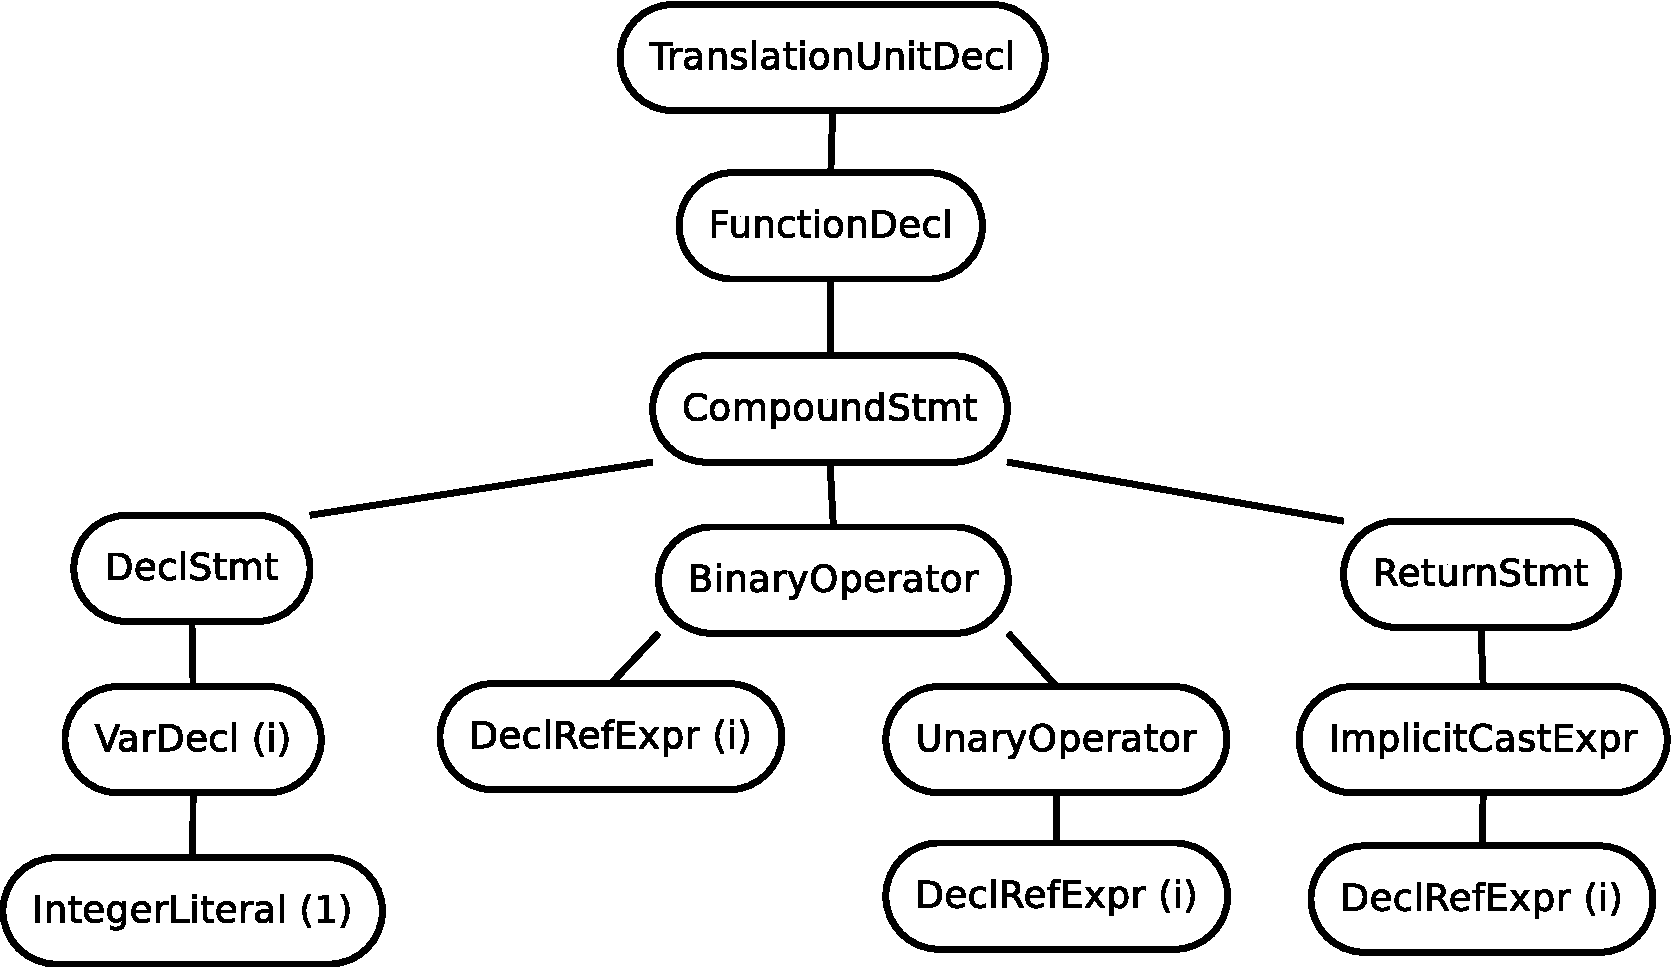
\includegraphics[width=1\textwidth]{fig/example1G.pdf}
\end{figure}

As we can see, we can, by definition of individual AST nodes, determine what (if any) child node is the side effect going to be applied to. Then when we go several levels up from node A towards the root and stop in node B, we can conclude that the whole subtree of B in which the node A is still has the side effect on the same memory address. We therefore can start from the DeclRefExpr nodes and while traversing the tree up to the root, decide whether the current node implies a side effect on a given DeclRefExpr.

%----------------------------------------------------------------------------------------------------------------
\subsection{L-value scope}
Some expressions keep an address of the given operand, meaning it can be used later in some parent node as an lvalue and, e.g., be assigned to. Consider this code:

\begin{lstlisting}
int main(void){
    int i = 2;
    int a = 3;
    *(a==3?&i:&i) = 42;
    return i;
}

\end{lstlisting}

In this example, it is the case of \verb|&i|. Some other expressions, however, get rid of the operand address irreversibly and we can be sure it will never be used as an L-value until its next occurence. An example of this is the \verb|b| variable in the conditional operator from the code above: it can never be used as an L-value in the whole subtree with the assignment it appears in as the conditional operator just uses it and throws it away.

%----------------------------------------------------------------------------------------------------------------
\subsection{Node tagging}
From this, we can conclude that every node can be tagged either as "implying a side effect", "not implying anything" or "making side effect impossible" on certain memory place given by certain DeclRefExpr. We can do this for each DeclRefExpr. The picture from the above would then be tagged as shown on figure \ref{ASTtagged}.
\begin{figure}
    \caption{Example 1~(\ref{example1}) AST graphical representation~--~tagged}
    \label{ASTtagged}
    \centering
        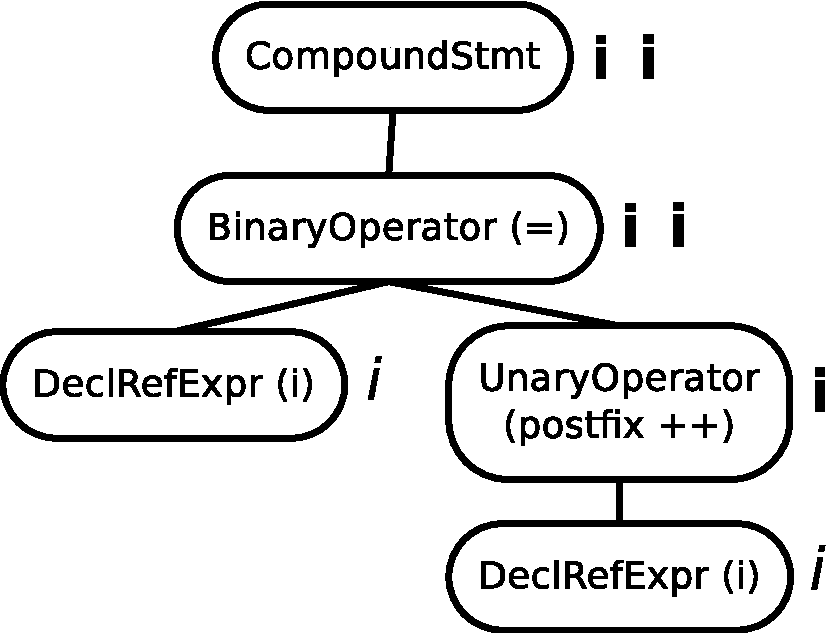
\includegraphics[width=0.6\textwidth]{fig/example1G-tagged.pdf}
\end{figure}

We began tagging from the left DeclRefExpr. It surely can be used as an L-value but the expression itself implies no side effect, hence the blue tag ("not implying anything"). We went towards the root and as we passed the \verb|BinaryExpression (=)|, we mark it as an expression implying a side effect on \verb|i| (red tag) as it modifies the memory contents of \verb|i|. We continued to the top implicitly marking all the parent nodes as having a side effect on \verb|i|. Then we can do the same for the right DeclRefExpr and as we see two red tags of the same variable, we can say we found an undefined behavior.

%TODO tabulka - co delam s jednotlivymi druhy uzlu?

%----------------------------------------------------------------------------------------------------------------
\subsection{Output of the first part}
For sake of portability, the output of the first phase is a plaintext directed to the standard output of the compiler. The output must contain the following information:

\begin{itemize}
\item Function in which the variables are to be checked for aliasing
\item Location of the statement with potentially undefined behavior
\item Variables to be checked; if they alias, undefined behavior occurs
\end{itemize}

Each possible undefined behavior is on one line. The format is
``\verb|function b_row b_col e_row e_col variable1 variable2|''
ff the constraint needs to be checked as \verb|variable1| and \verb|variable2| are different, or
``\verb|function b_row b_col e_row e_col variable|''
if no further check is needed as the possible undefined behavior comes from occurences of the same variable. \verb|b_row| and \verb|b_col| denote the row and columnt of the beginning of statement the undefined behavior occurs in and \verb|e_row| and \verb|e_col| denote its end.

\begin{figure}
\caption{Output of the first part of the SPA}
\label{first-part-output}
\begin{lstlisting}
main 16 9 16 19 *j *k
main 16 9 16 19 *k *j
main 16 5 16 19 *j i
main 16 5 16 19 *k i
\end{lstlisting}
\end{figure}

This output can then be used by any external alias analysis.

%================================================================================================================
\section{Checking the constraints}
Once the constraints are generated, there are many means of checking them. Any alias analysis may be used and it is the alias analysis used what decides an algorithm used for comparing it with the constraints as the output and information received from the alias analysis may vary for each implementation. We will further describe our actual implementation which is a bash script using a built-in alias analysis of the LLVM. We will use the example \ref{example2} (\verb|i = (*1)++|) for rhe following examples.

%----------------------------------------------------------------------------------------------------------------
\subsection{Alias analysis implementation}
We used the alias analysis implemented in the LLVM. It offers multiple versions of alias analysis and after testing, the ``basic'' alias analysis was evaluated as best. This implementation of alias analysis is simple and leads to many indefinite answers but in our case, it led to at least some results while other implementations seemed absolutely useless. Considering our approach to indefinite answers mentioned later and the results of the tests, the ``basic'' version seems to be absolutely sufficient.

Other implementations' failures were probably caused by the fact that they depend heavily on compiler optimizations~\cite{alias-analysis-optimizations} which, however, need to be turned off completely. Searching for aliases in the optimized code and trying to match them to the original source would make no sense. Testing shows that in many cases, the alias analysis would just stop with a ``no pointers'' error meaning anything that could be checked has been optimized out.

%----------------------------------------------------------------------------------------------------------------
\subsection{Output of the alias analysis}
Figure \ref{alias-output} shows part of the output of alias analysis of the example \ref{example2}. We can easily filter out the non-aliasing variables. Out of possible answers~--~NoAlias, MayAlias, MustAlias~--~the latter two are considered to confirm that an undefined behavior occurs. This may lead to false positives depending on alias analysis used~--~MayAlias is not a definite answer and we simply choose possible false positives over false negatives.

We see there are many temporary variables (the numbered ones) and not the original names of the variables. In order to match these temporary variables to real variable names, we need the LLVM IR of the original program.

The alias analysis can be run on the LLVM IR (``intermediate representation'', ``bitcode''), which can also be printed as a text and also can contain debug info. These three things are necessary for the following approach to work.
\begin{figure}
\caption{Output of the alias analysis}
\label{alias-output}
\begin{lstlisting}
$ opt -disable-output -basicaa --aa-eval -print-all-alias-modref-info test1A.bc 
Function: main: 4 pointers, 2 call sites
  NoAlias:	i32* %i, i32* %retval
  NoAlias:	i32* %retval, i32** %j
  NoAlias:	i32* %i, i32** %j
  NoAlias:	i32* %0, i32* %retval
  MayAlias:	i32* %0, i32* %i
  NoAlias:	i32* %0, i32** %j
\end{lstlisting}
\end{figure}

%----------------------------------------------------------------------------------------------------------------
\subsection{Alias translation}
On figure \ref{llvmir}, there is a part of the LLVM IR necessary for translation of the temporary variables to their original names. On that example, we can see that \verb|\%0| matches \verb|*j| in the original source file.

Furthermore, we can see a link to debuginfo \verb|!dbg !19| attached which can be used in the next part.
\begin{figure}
\caption{LLVM IR}
\label{llvmir}
\begin{lstlisting}
$ llvm-dis test1A.bc -o -
define i32 @main() #0 {
  call void @llvm.dbg.declare(metadata !{i32* %i}, metadata !12), !dbg !13
  store i32 0, i32* %i, align 4, !dbg !14
  call void @llvm.dbg.declare(metadata !{i32** %j}, metadata !15), !dbg !17
  store i32* %i, i32** %j, align 8, !dbg !18
  %0 = load i32** %j, align 8, !dbg !19
  %1 = load i32* %0, align 4, !dbg !19
  %inc = add nsw i32 %1, 1, !dbg !19
  store i32 %inc, i32* %0, align 4, !dbg !19
  store i32 %1, i32* %i, align 4, !dbg !19
  %2 = load i32* %i, align 4, !dbg !20
  ret i32 %2, !dbg !20
\end{lstlisting}
\end{figure}

For multiple functions, the results are similar and LLVM IR keeps the division into function so we are able to filter out all the functions we do not currently want to match against. This is important because temporary variable names are not unique across functions.

%----------------------------------------------------------------------------------------------------------------
\subsection{Matching translated aliases to their original location}
Figure \ref{debuginfo} shows the debug info necessary to match the aliasing info to the original source code. Using the link to debug info from a LLVM IR, we can find the correct debug info which contains information on location in the source file and the function name. The row is the first argument, the column the second argument and the third argument is a link to another debug info (in this case \verb|!dbg !4|) which contains information about the function the undefined behavior occurs in.

\begin{figure}
\caption{Debug info}
\label{debuginfo}
\begin{lstlisting}
$ llvm-dis test1A.bc -o -
!0 = metadata !{i32 786449, metadata !1, i32 12, metadata !"clang version 3.5.0 (trunk 205669)", i1 false, metadata !"", i32 0, metadata !2, metadata !2, metadata !3, metadata !2, metadata !2, metadata !"", i32 1} ; [ DW_TAG_compile_unit ] [/home/lhellebr/bc/new/SPA/SPA/examples/test1A.c] [DW_LANG_C99]
!1 = metadata !{metadata !"SPA/examples/test1A.c", metadata !"/home/lhellebr/bc/new/SPA"}
!2 = metadata !{}
!3 = metadata !{metadata !4}
!4 = metadata !{i32 786478, metadata !1, metadata !5, metadata !"main", metadata !"main", metadata !"", i32 3, metadata !6, i1 false, i1 true, i32 0, i32 0, null, i32 0, i1 false, i32 ()* @main, null, null, metadata !2, i32 3} ; [ DW_TAG_subprogram ] [line 3] [def] [main]
!5 = metadata !{i32 786473, metadata !1}          ; [ DW_TAG_file_type ] [/home/lhellebr/bc/new/SPA/SPA/examples/test1A.c]
!6 = metadata !{i32 786453, i32 0, null, metadata !"", i32 0, i64 0, i64 0, i64 0, i32 0, null, metadata !7, i32 0, null, null, null} ; [ DW_TAG_subroutine_type ] [line 0, size 0, align 0, offset 0] [from ]
!7 = metadata !{metadata !8}
!8 = metadata !{i32 786468, null, null, metadata !"int", i32 0, i64 32, i64 32, i64 0, i32 0, i32 5} ; [ DW_TAG_base_type ] [int] [line 0, size 32, align 32, offset 0, enc DW_ATE_signed]
!9 = metadata !{i32 2, metadata !"Dwarf Version", i32 4}
!10 = metadata !{i32 1, metadata !"Debug Info Version", i32 1}
!11 = metadata !{metadata !"clang version 3.5.0 (trunk 205669)"}
!12 = metadata !{i32 786688, metadata !4, metadata !"i", metadata !5, i32 4, metadata !8, i32 0, i32 0} ; [ DW_TAG_auto_variable ] [i] [line 4]
!13 = metadata !{i32 4, i32 7, metadata !4, null}
!14 = metadata !{i32 4, i32 3, metadata !4, null}
!15 = metadata !{i32 786688, metadata !4, metadata !"j", metadata !5, i32 5, metadata !16, i32 0, i32 0} ; [ DW_TAG_auto_variable ] [j] [line 5]
!16 = metadata !{i32 786447, null, null, metadata !"", i32 0, i64 64, i64 64, i64 0, i32 0, metadata !8} ; [ DW_TAG_pointer_type ] [line 0, size 64, align 64, offset 0] [from int]
!17 = metadata !{i32 5, i32 8, metadata !4, null}
!18 = metadata !{i32 5, i32 3, metadata !4, null}
!19 = metadata !{i32 6, i32 3, metadata !4, null}
!20 = metadata !{i32 7, i32 3, metadata !4, null}
\end{lstlisting}
\end{figure}

In order to get access to this debug info, we need to compile to the bitcode using \verb|-g3| (for debug info in general) and \verb|-gcolumn-info| (for columnt information, otherwise it would be always 0 for performance reasons) parameters.
%----------------------------------------------------------------------------------------------------------------
\subsection{Constraints and translated aliases comparison}\label{flaw}
The described method will lead to a set of constraints from the first part of the SPA (figure \ref{first-part-output}) \emph{and} a set of aliases matched with their original names and locations (``translated aliases''). It is then a matter of comparing two lists, each item with each, and if some of them matches, it indicates the undefined behavior.

As we found no way of getting the exact position of the \emph{statement} where two variables alias out of the LLVM alias analysis, we need to introduce a solution possibly leading to false positives: If two variables have aliased \emph{anywhere before the statement, and in the same function as the statement occurs}, it is considered to alias in that statement, too. This is a flaw we were not able to circumvent. Example of this case is in figure \ref{example-alias-before}, where \verb|*k| is considered as aliasing with \verb|i| and undefined behavior is falsely detected. This is a flaw of the second part of the SPA and depends on information accessible from the alias analysis. Alias analysis errors and indefinite answers may also lead to false positives.
\begin{figure}
\caption{False positive example}
\label{example-alias-before}
\begin{lstlisting}
int main(void){
  int i = 42, j = 42;
  int *k = &i;
  k = &j;
  i = (*k)++;
  return i;
}
\end{lstlisting}
\end{figure}
%----------------------------------------------------------------------------------------------------------------
\subsection{Output format}
The output of the second part is meant to be the final output of the SPA for the user. It shows actual undefined behavior occurences (in contrast with the first part showing all \emph{possible} occurences), the function name, the \emph{approximate position} and names of the variable(s) causing the undefined behavior.

Example output:
\begin{lstlisting}
Possible undefined behavior in function "main" at [16,9] - "*j" aliases with "*k"
Possible undefined behavior in function "main" at [16,5] - "*j" aliases with "i"
Possible undefined behavior in function "main" at [16,5] - "*k" aliases with "i"
\end{lstlisting}

%%%%%%%%%%%%%%%%%%%%%%%%%%%%%%%%%%%%%%%%%%%%%%%%%%%%%%%%%%%%%%%%%%%%%%%%%%%%%%%%%%%%%%%%%%%%%%%%%%%%%%%%%%%%%%%%%
\chapter{Implementation and testing}
In this chapter, we will briefly describe the implementation and show tests and their results.
%================================================================================================================
\section{Implementation}
The project consists of: \verb|Makefile|, the Clang plugin part (\verb|SPA.cpp|, \verb|LvalueTable.cpp|), alias analysis part (\verb|run.sh| and \verb|debugrun.sh| bash scripts), and support files like documentation and examples.

The Makefile is written so that it automatically downloads latest versions of all the necessary software, such as Clang or LLVM, and installs them together with SPA in the current directory.

The Clang plugin part consists of two \verb|.cpp| files. For implementation reasons, there are no header files. The \verb|SPA.cpp| file consists of the part connecting the SPA with Clang and of the part traversing the AST and deciding what node should be tagged. The \verb|LvalueTable.cpp| file provides functions for actual tagging of nodes and generating the final constraints.

The alias analysis part is a Bash script \verb|run.sh| that uses the output of the first part, and together with LLVM IR, alias analysis output and debug info checks the constraints and provides the final output to the user. The \verb|run.sh| script is what user invokes directly. There is also a \verb|debugrun.sh| file automatically generated from a \verb|run.sh| file during a \verb|make| command, that shows The constraints, LLVM IR, debug info, alias analysis output and the final output rather than only the final output. See the example debug output in the figure \ref{debug}.

The documentation source files in latex are in a \verb|SPA/doc| folder, the installation instructions are in \verb|INSTALL.txt| and very basic info about the SPA is in \verb|README.md|.

\begin{figure}
\caption{Debug output}
\label{debug}
\begin{lstlisting}
$ ./debugrun.sh SPA/examples/test1A.c
LLVM IR:
define i32 @main() #0 {
  call void @llvm.dbg.declare(metadata !{i32* %i}, metadata !12), !dbg !13
  store i32 0, i32* %i, align 4, !dbg !14
  call void @llvm.dbg.declare(metadata !{i32** %j}, metadata !15), !dbg !17
  store i32* %i, i32** %j, align 8, !dbg !18
  %0 = load i32** %j, align 8, !dbg !19
  %1 = load i32* %0, align 4, !dbg !19
  %inc = add nsw i32 %1, 1, !dbg !19
  store i32 %inc, i32* %0, align 4, !dbg !19
  store i32 %1, i32* %i, align 4, !dbg !19
  %2 = load i32* %i, align 4, !dbg !20
  ret i32 %2, !dbg !20
!0 = metadata !{i32 786449, metadata !1, i32 12, metadata !"clang version 3.5.0 (trunk 205669)", i1 false, metadata !"", i32 0, metadata !2, metadata !2, metadata !3, metadata !2, metadata !2, metadata !"", i32 1} ; [ DW_TAG_compile_unit ] [/home/lhellebr/bc/new/SPA/SPA/examples/test1A.c] [DW_LANG_C99]
!1 = metadata !{metadata !"SPA/examples/test1A.c", metadata !"/home/lhellebr/bc/new/SPA"}
!2 = metadata !{}
!3 = metadata !{metadata !4}
!4 = metadata !{i32 786478, metadata !1, metadata !5, metadata !"main", metadata !"main", metadata !"", i32 3, metadata !6, i1 false, i1 true, i32 0, i32 0, null, i32 0, i1 false, i32 ()* @main, null, null, metadata !2, i32 3} ; [ DW_TAG_subprogram ] [line 3] [def] [main]
!5 = metadata !{i32 786473, metadata !1}          ; [ DW_TAG_file_type ] [/home/lhellebr/bc/new/SPA/SPA/examples/test1A.c]
!6 = metadata !{i32 786453, i32 0, null, metadata !"", i32 0, i64 0, i64 0, i64 0, i32 0, null, metadata !7, i32 0, null, null, null} ; [ DW_TAG_subroutine_type ] [line 0, size 0, align 0, offset 0] [from ]
!7 = metadata !{metadata !8}
!8 = metadata !{i32 786468, null, null, metadata !"int", i32 0, i64 32, i64 32, i64 0, i32 0, i32 5} ; [ DW_TAG_base_type ] [int] [line 0, size 32, align 32, offset 0, enc DW_ATE_signed]
!9 = metadata !{i32 2, metadata !"Dwarf Version", i32 4}
!10 = metadata !{i32 1, metadata !"Debug Info Version", i32 1}
!11 = metadata !{metadata !"clang version 3.5.0 (trunk 205669)"}
!12 = metadata !{i32 786688, metadata !4, metadata !"i", metadata !5, i32 4, metadata !8, i32 0, i32 0} ; [ DW_TAG_auto_variable ] [i] [line 4]
!13 = metadata !{i32 4, i32 7, metadata !4, null}
!14 = metadata !{i32 4, i32 3, metadata !4, null}
!15 = metadata !{i32 786688, metadata !4, metadata !"j", metadata !5, i32 5, metadata !16, i32 0, i32 0} ; [ DW_TAG_auto_variable ] [j] [line 5]
!16 = metadata !{i32 786447, null, null, metadata !"", i32 0, i64 64, i64 64, i64 0, i32 0, metadata !8} ; [ DW_TAG_pointer_type ] [line 0, size 64, align 64, offset 0] [from int]
!17 = metadata !{i32 5, i32 8, metadata !4, null}
!18 = metadata !{i32 5, i32 3, metadata !4, null}
!19 = metadata !{i32 6, i32 3, metadata !4, null}
!20 = metadata !{i32 7, i32 3, metadata !4, null}

Aliases:
main 0 i

Constraints:
main 6 3 6 3 *j i

Translated aliases:
main 6 3 any any *j i

Results:
Possible undefined behavior in function "main" at [6,3] - "*j" aliases with "i"
\end{lstlisting}
\end{figure}
%----------------------------------------------------------------------------------------------------------------
\subsection{Further development}
Here we discuss the SPA's potential for further development and possible usability for upstream.

The first part is a Clang plugin. As any other Clang plugin, it uses an interface that is \emph{not considered stable}~\cite{clang-unstable} and would need to be consistently developed should it be a par of upstream. The plugin itself works well and may serve as a starting point for further development.

The second part is not as rigid as the first one. It can be easily replaced by some other script using some other alias analysis implementation. It has a flaw described in \ref{flaw}. It relies on exact output format of alias analysis which is, however, not considered stable. This part is innovative in means of mapping the original variable name and location to a temporary variable via debug info, but should not be considered stable nor should any further development be based on it.

As to including the whole SPA to upstream, there is generally one issue that makes it difficult and arguably useless: it doesn't find the final results during the compilation. It merely generates constraints which need to be further checked, that is what \verb|run.sh| does. That means this check can't be transparently added to the Clang compile-time checks without major changes in the Clang's architecture.

Potential further development, other than debugging, is thus making the whole tool invokable just as a Clang plugin.
%================================================================================================================
\section{Testing}
We will test the application using a prepared set of testcases. These can also be effectively used as demonstration of the undefined behavior problem and the principles of the SPA.
In this section, we will describe testcases and statistically analyze the results.
%----------------------------------------------------------------------------------------------------------------
\subsection{Testcases}
Currently there are 21 tests. Some of them use pointers. Results of some of them are expected to be positive (undefined behavior found), some are expected to be negative. See details in the table:\\

\begin{tabular}{|l|l|l|}
\hline
                 & Positive & Negative \\\hline
With pointers    & 7        & 3        \\\hline
Without pointers & 9        & 2        \\\hline
\end{tabular}\\

The tests vary in constructions used, use different data types, statement types and undefined behavior origins. Most of them are in a pointer and non-pointer version. They are part of both the repository and the attached source codes.

Some of these cases are: undefined behavior while indexing arrays, functions, ignoring compound statements, correct resolving of sequence points in a ternary operator, tricks to make alias analysis fail, etc.

%----------------------------------------------------------------------------------------------------------------
\subsection{Test results}

The results are shown in the following table:

\begin{tabular}{|r|r|}
\hline
True Positives                         &             16   \\\hline
True Negatives                         &              4   \\\hline
False Positives                        &              1   \\\hline
False Negatives                        &              0   \\\hline\hline
\textbf{Sensitivity}                   & \textbf{100\%}   \\\hline
\textbf{Specificity}                   &  \textbf{80\%}   \\\hline
Fall-out                               &           20\%   \\\hline
\textbf{Positive predictive value}     &  \textbf{94\%}   \\\hline
\textbf{Negative predictive value}     & \textbf{100\%}   \\\hline
False discovery rate                   &            6\%   \\\hline\hline
\textbf{Accuracy}                      &  \textbf{95\%}   \\\hline
F1 score                               &           97\%   \\\hline
\end{tabular}\\

As we can see, there were no false negatives, which means that the SPA never ``missed'' an actual undefined behavior. In this test set, we have found one false positive. This false positive was caused by the second phase and is caused by the flaw described in the second paragraph of \ref{flaw}. The test was created with this flaw specifically in mind.

After some statistical analysis, we see that, based on this test set, if there is no undefined behavior detected, there is certainly no undefined behavior (related to sequence points and side effects) and if there is some undefined behavior detected, there is a 94\% chance there actually is undefined behavior.

The overall accuracy of the SPA is 95\% and the only error in the set is caused by the second phase of the SPA.

%%%%%%%%%%%%%%%%%%%%%%%%%%%%%%%%%%%%%%%%%%%%%%%%%%%%%%%%%%%%%%%%%%%%%%%%%%%%%%%%%%%%%%%%%%%%%%%%%%%%%%%%%%%%%%%%%
\chapter{Installation and usage}
In this chapter, we will discuss the software requirements of the SPA, its automated installation and manual installation. We will discuss the usage from user's point of view.%TODO and show and example
%================================================================================================================
\section{Requirements}
The tool should run on any system capable of compiling and running LLVM and Clang \emph{and} invoking a Bash script in POSIX environment. It has been tested on Linux, specifically multiple versions of Fedora 17 and 19, both x86\_64 architecture.

Clang is only required for the first part and full LLVM for the second part. The SPA uses the interfaces of Clang and LLVM that are both considered unstable so it might require specific versions of these tools. It has been tested on Clang 3.5.0  and LLVM 3.5.0.

The best way to download the SPA is Git. The Makefile itself uses SVN which is therefore required for the automated installation.
%================================================================================================================
\section{Installation}
\begin{enumerate}
\item If you do not have the SPA, you need to download it, for example by
\begin{verbatim}git clone https://github.com/KamikazeCZ/SPA.git\end{verbatim}

\item Go to the newly created repository directory

\item For automated installation, run
\begin{verbatim}make\end{verbatim}
\end{enumerate}
%================================================================================================================
\section{Manual installation}
For manual installation, you need to download Clang and LLVM. Refer to points 1 to 5 of the Get Started guide~\cite{clang-get_started}. You do not need Clang extra tools.

After following these instructions, you should have a \verb|llvm| directory with the source of both LLVM and Clang. Copy the SPA folder (the one \emph{inside} the repository) to \verb|llvm/tools/clang/tools|. Also copy the \verb|SPA/top-level-makefile/Makefile| file to \verb|llvm/tools/clang/tools|.

This should have added the SPA as a Clang plugin and you can continue by point 6 of the Get Started guide.
%================================================================================================================
\section{Usage}
To verify the correct installation, run \begin{verbatim}make run\end{verbatim} This is equivalent to running \begin{verbatim}./run SPA/examples/test1A.c\end{verbatim}

Running \verb|./run <file.c>| is a standard way to run the whole SPA on certain file. It is a script executing both parts of the SPA. To only run the first part, run \begin{verbatim}build/Release+Asserts/bin/clang <file.c>\end{verbatim}
For debug mode, use \begin{verbatim}./debugrun <file.c>\end{verbatim} instead.

To generate this documentation, run \verb|make| in \verb|SPA/doc|.
%%%%%%%%%%%%%%%%%%%%%%%%%%%%%%%%%%%%%%%%%%%%%%%%%%%%%%%%%%%%%%%%%%%%%%%%%%%%%%%%%%%%%%%%%%%%%%%%%%%%%%%%%%%%%%%%%
\chapter{Conclusion}
A tool has been implemented that searches for undefined behavior related to side effects and sequence points in the C language programs. It consists of two parts, the first part generates a list of \emph{possible} undefined behavior occurences and the second part verifies these constraints and generates the final user-readable output. The first part is implemented as a Clang plugin, the second as a Bash script using alias analysis in LLVM.

The tests have shown the accuracy of 95\%, positive predictive value of 94\% and negative predictive value of 100\%. The only failed test failed due to the known flaw  originating in alias analysis giving not enough information.

The tool is currently probably not useful in the upstream due to its two-phase architecture which doesn't allow for transparent compile-time checks in Clang. It can be, however, used as a starting point for further development, particularly its first part which seems to work well.
 % viz. obsah.tex

  % Pouzita literatura
  % ----------------------------------------------
\ifczech
  \bibliographystyle{czechiso}
\else 
  \bibliographystyle{plain}
%  \bibliographystyle{alpha}
\fi
  \begin{flushleft}
  \bibliography{literatura} % viz. literatura.bib
  \end{flushleft}
  \appendix
  
  \chapter{DVD contents}
The DVD contains exactly the same content as the git repository at the time of burning the DVD. The only difference is that it also contains this documentation in pdf. The directory structure is as follows:

\begin{itemize}
\item Makefile -- the only thing you should need to make the whole tool running
\item README.md and INSTALL.txt -- basic information about the tool and the installation instructions
\item SPA -- the source files
  \begin{itemize}
  \item doc -- the source files for generating this documentation
  \item examples -- the source files of tests/examples
    \begin{itemize}
      \item negative -- the source files of tests that are not supposed to find any undefined behavior
    \end{itemize}
  \item SPA.cpp, LvalueTable.cpp, run.sh -- the source code of the tool itself, as described in the ``Implementation and testing'' chapter
  \end{itemize}
\item projekt.pdf -- this documentation
\end{itemize}

%%%%%%%%%%%%%%%%%%%%%%%%%%%%%%%%%%%%%%%%%%%%%%%%%%%%%%%%%%%%%%%%%%%%%%%%%%%%%%%%%%%%%%%%%%%%%%%%%%%%%%%%%%%%%%%%%
\chapter{Installation and usage}
In this chapter, we will discuss the software requirements of the SPA, its automated installation and manual installation. We will discuss the usage from user's point of view.%TODO and show and example
%================================================================================================================
\section{Requirements}
The tool should run on any system capable of compiling and running LLVM and Clang \emph{and} invoking a Bash script in POSIX environment. It has been tested on Linux, specifically multiple versions of Fedora 17 and 19, both x86\_64 architecture.

Clang is only required for the first part and full LLVM for the second part. The SPA uses the interfaces of Clang and LLVM that are both considered unstable so it might require specific versions of these tools. It has been tested on Clang 3.5.0  and LLVM 3.5.0.

The best way to download the SPA is Git. The Makefile itself uses SVN which is therefore required for the automated installation.
%================================================================================================================
\section{Installation}
\begin{enumerate}
\item If you do not have the SPA, you need to download it, for example by
\begin{verbatim}git clone https://github.com/KamikazeCZ/SPA.git\end{verbatim}

\item Go to the newly created repository directory

\item For automated installation, run
\begin{verbatim}make\end{verbatim}
\end{enumerate}
%================================================================================================================
\section{Manual installation}
For manual installation, you need to download Clang and LLVM. Refer to points 1 to 5 of the Get Started guide~\cite{clang-get_started}. You do not need Clang extra tools.

After following these instructions, you should have a \verb|llvm| directory with the source of both LLVM and Clang. Copy the SPA folder (the one \emph{inside} the repository) to \verb|llvm/tools/clang/tools|. Also copy the \verb|SPA/top-level-makefile/Makefile| file to \verb|llvm/tools/clang/tools|.

This should have added the SPA as a Clang plugin and you can continue by point 6 of the Get Started guide.
%================================================================================================================
\section{Usage}
To verify the correct installation, run \begin{verbatim}make run\end{verbatim} This is equivalent to running \begin{verbatim}./run SPA/examples/test1A.c\end{verbatim}

Running \verb|./run <file.c>| is a standard way to run the whole SPA on certain file. It is a script executing both parts of the SPA. To only run the first part, run \begin{verbatim}build/Release+Asserts/bin/clang <file.c>\end{verbatim}
For debug mode, use \begin{verbatim}./debugrun <file.c>\end{verbatim} instead.

To generate this documentation, run \verb|make| in \verb|SPA/doc|.
 % viz. prilohy.tex
\end{document}
